\documentclass[12pt]{beamer}

%  CORE PACKAGES --------------------------------
\usepackage{amsmath, amssymb, graphicx, booktabs, tabularx, setspace, soul}
\usepackage{subcaption}
\usepackage{tikz, pgfplots}
\pgfplotsset{compat=1.18}
\usetikzlibrary{positioning, arrows.meta, arrows.meta, positioning, shapes, calc}
\usepackage[many]{tcolorbox}
\usepackage[ruled,vlined]{algorithm2e}
\usepackage{minted}

%  FONTS & STYLING ------------------------------
\usepackage{fontspec}
\usefonttheme{professionalfonts}
\setsansfont[
UprightFont     = *Light,
BoldFont        = *Bold,
ItalicFont      = *Light Italic,
BoldItalicFont  = *Bold Italic,
Ligatures       = TeX,
Scale           = MatchLowercase
]{Frutiger LT Pro}
\renewcommand{\familydefault}{\sfdefault}
\linespread{1.}\selectfont
\hyphenpenalty=10000
\exhyphenpenalty=10000

%  COLORS & THEMES ------------------------------
\definecolor{aggiemaroon}{RGB}{80,0,0}
\definecolor{beamer@blendedblue}{RGB}{80,0,0}
\usecolortheme{default}

\setbeamertemplate{itemize items}{•}
\setbeamertemplate{itemize subitem}[•]
\setbeamertemplate{itemize subsubitem}[•]
\renewcommand{\UrlFont}{\ttfamily\small}

%  HYPERLINKS -----------------------------------
\usepackage{hyperref}
\hypersetup{
colorlinks=true,
linkcolor=aggiemaroon,
urlcolor=aggiemaroon,
citecolor=aggiemaroon
}

%  BEAMER TEMPLATES -----------------------------
\setbeamertemplate{caption}[numbered]
\setbeamertemplate{navigation symbols}{}
\setbeamertemplate{footline}{
\color{aggiemaroon}{\hfill \insertframenumber/\inserttotalframenumber \hspace{2pt} \vskip2pt}
}

%  CUSTOM ENVIRONMENTS --------------------------
\newenvironment{stepenumerate}{
\begin{enumerate}[<+->]
}{\end{enumerate}}

\newenvironment{stepitemize}{
\begin{itemize}[<+->]
}{\end{itemize}}

\newenvironment{stepenumeratewithalert}{
\begin{enumerate}[<+-| alert@+>]
}{\end{enumerate}}

\newenvironment{stepitemizewithalert}{
\begin{itemize}[<+-| alert@+>]
}{\end{itemize}}

% DOCUMENT INFO ---------------------------------
\title{Decision and Risk Analysis}
\subtitle{Lecture 2: \textbf{Bayes’ Rule}}
\author{\emph{}}
\date{\color{aggiemaroon}{
DAEN 427/ISEN 427/ISEN 627\\
\textbf{Alexander Abuabara}\\
Fall 2026
}}
\titlegraphic{\vfill 
\includegraphics[height=1.2cm]{TAMU_logo.png}}

% -----------------------------------------------
\begin{document}

% -----------------------------------------------
\maketitle

%------------------------------------------------
\begin{frame}{}
\begin{columns}[c]
% Left column: image
    \begin{column}{0.32\textwidth}
    \centering
    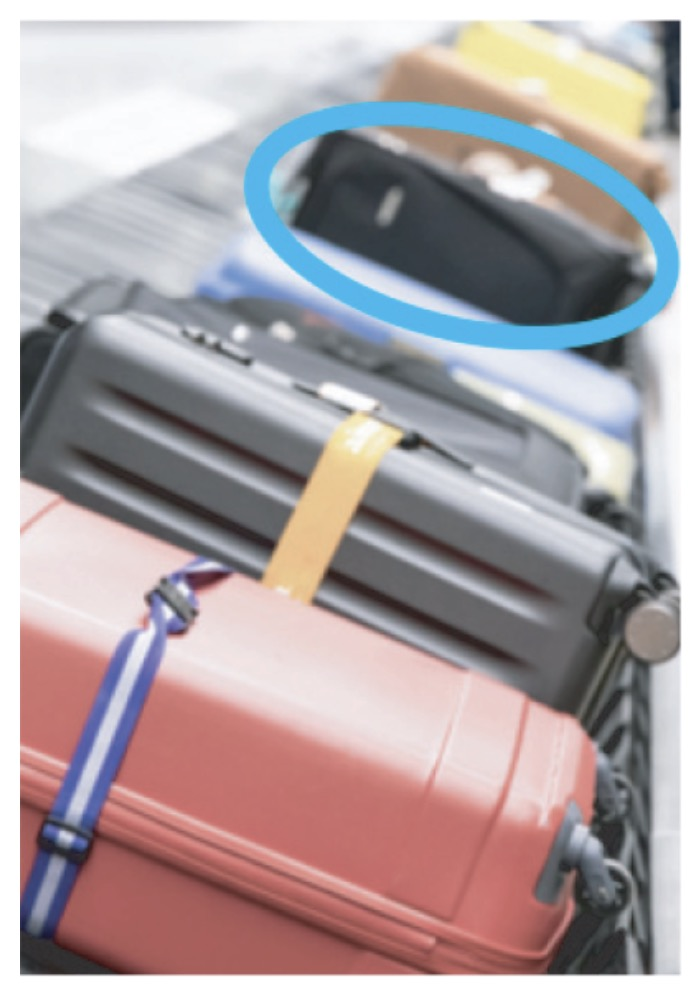
\includegraphics[width=3.75cm]{Bags.jpg}
    \end{column}
% Right column: text
    \begin{column}{0.66\textwidth}
    \small
    Let's suppose that you are an air traveler along with 99 other passengers from your flight, each of whom, like you, checked one item of luggage.
    
    \vspace{0.2cm}
    
    A recording piped through the speakers reminds you that:
    \emph{``Many bags look alike. Please check your bag carefully before exiting the terminal.''}
    
    \vspace{0.2cm}
    
    Indeed, your bag is one of the most popular models on the market, a medium-sized black rectangular case \textbf{used by 5\% of all travelers}.
    
    \vspace{0.2cm}
    
    Given your distance from the luggage chute, you can discern only the shape, size, and color of the bags that emerge, not any detailed markings on the bags.
    \end{column}
\end{columns}
\end{frame}

%------------------------------------------------
\begin{frame}{}
\begin{itemize}
\item[a.] Let's suppose that the \textbf{first bag} from your flight to enter the luggage carousel indeed has the same shape, size, and color as yours.
          Is it yours? Explain (i.e., calculate the posterior probability that the 1st bag is yours).

\vspace{0.4cm}
    
\item[b.] Now suppose that we continue to wait for our bag to appear, failing to see it among the first 98 bags to enter the carousel (i.e., only 2 bags are left to come off the airplane).
          Calculate the posterior probability that the \textbf{99th} bag, which also matches ours in shape, size, and color, is our own.
\end{itemize}
\end{frame}

%------------------------------------------------
\begin{frame}{We’re Using R Instead of Python}
\begin{block}{Python}
\begin{itemize}
\item "Can do everything" ... installs $n$ packages, breaks after update
\item Stack Overflow becomes your TA
\end{itemize}
\end{block}
\begin{block}{R}
\begin{itemize}
\item Literally for statistics: \texttt{lm(y \textasciitilde{} x)} and move on with your life
\item Excellent, open-source, keeps us focused on data analysis,\\and I enjoy sleeping at night!
\end{itemize}
\end{block}
\textbf{What I Need From You:} learn concepts, analyze data, pass the class.\\
\textbf{What I Do Not Need:} a 2-hour debate about virtual environments.

\end{frame}

%------------------------------------------------
\begin{frame}[fragile]{}

\begin{minted}[fontsize=\footnotesize, linenos]{r}
# Load packages
library(bayesrules)
library(tidyverse)
library(janitor)

# Import article data
data(fake_news)

fake_news %>% 
  tabyl(type) %>% 
  adorn_totals("row")
#  type   n percent
#  fake  60     0.4
#  real  90     0.6
# Total 150     1.0
\end{minted}

\end{frame}

%------------------------------------------------
\begin{frame}{Building a Bayesian Model for Events}
\begin{block}{Prior Probability Model}
\begin{itemize}
\item 
\item 
\item 
\end{itemize}
\end{block}
\end{frame}

%------------------------------------------------
\begin{frame}{}
\begin{block}{Conditional Probability \& Likelihood}
\begin{itemize}
\item 
\item 
\item 
\end{itemize}
\end{block}
\end{frame}

%------------------------------------------------
\begin{frame}{}
\begin{block}{Conditional vs Unconditional Probability}
\begin{itemize}
\item 
\item 
\item 
\end{itemize}
\end{block}
\end{frame}

%------------------------------------------------
\begin{frame}{}
\begin{block}{Independent Events}
\begin{itemize}
\item 
\item 
\item 
\end{itemize}
\end{block}
\end{frame}

%------------------------------------------------
\begin{frame}{}
\begin{block}{Probability vs Likelihood}
\begin{itemize}
\item 
\item 
\item 
\end{itemize}
\end{block}
\end{frame}

%------------------------------------------------
\begin{frame}{}
\begin{block}{Normalizing Constants}
\begin{itemize}
\item 
\item 
\item 
\end{itemize}
\end{block}
\end{frame}

%------------------------------------------------
\begin{frame}{}
\begin{block}{Calculating Joint and Conditional Probabilities}
\begin{itemize}
\item 
\item 
\item 
\end{itemize}
\end{block}
\end{frame}

%------------------------------------------------
\begin{frame}{}
\begin{block}{Posterior Probability Model via Bayes’ Rule}
\begin{itemize}
\item 
\item 
\item 
\end{itemize}
\end{block}
\end{frame}

%------------------------------------------------
\begin{frame}{}
\begin{block}{Posterior Simulation}
\begin{itemize}
\item 
\item 
\item 
\end{itemize}
\end{block}
\end{frame}

%------------------------------------------------
\begin{frame}{Building a Bayesian Model for Random Variables}
\begin{block}{Prior Probability Model}
\begin{itemize}
\item 
\item 
\item 
\end{itemize}
\end{block}
\end{frame}

%------------------------------------------------
\begin{frame}{}
\begin{block}{Discrete Probability Model}
\begin{itemize}
\item 
\item 
\item 
\end{itemize}
\end{block}
\end{frame}

%------------------------------------------------
\begin{frame}{}
\begin{block}{The Binomial Data Model}
\begin{itemize}
\item 
\item 
\item 
\end{itemize}
\end{block}
\end{frame}

%------------------------------------------------
\begin{frame}{}
\begin{block}{Conditional Probability Model of Data $Y$}
\begin{itemize}
\item 
\item 
\item 
\end{itemize}
\end{block}
\end{frame}

%------------------------------------------------
\begin{frame}{}
\begin{block}{The Binomial Model}
\begin{itemize}
\item 
\item 
\item 
\end{itemize}
\end{block}
\end{frame}

%------------------------------------------------
\begin{frame}{}
\begin{block}{The Binomial Likelihood Function}
\begin{itemize}
\item 
\item 
\item 
\end{itemize}
\end{block}
\end{frame}

%------------------------------------------------
\begin{frame}{}
\begin{block}{Probability Mass Functions vs Likelihood Functions}
\begin{itemize}
\item 
\item 
\item 
\end{itemize}
\end{block}
\end{frame}

%------------------------------------------------
\begin{frame}{}
\begin{block}{Normalizing Constant}
\begin{itemize}
\item 
\item 
\item 
\end{itemize}
\end{block}
\end{frame}

%------------------------------------------------
\begin{frame}{}
\begin{block}{Posterior Probability Model}
\begin{itemize}
\item 
\item 
\item 
\end{itemize}
\end{block}
\end{frame}

%------------------------------------------------
\begin{frame}{}
\begin{block}{Bayes’ Rule for Variables}
\begin{itemize}
\item 
\item 
\item 
\end{itemize}
\end{block}
\end{frame}

%------------------------------------------------
\begin{frame}{}
\begin{block}{Posterior Shortcut}
\begin{itemize}
\item 
\item 
\item 
\end{itemize}
\end{block}
\end{frame}

%------------------------------------------------
\begin{frame}{}
\begin{block}{Proportionality}
\begin{itemize}
\item 
\item 
\item 
\end{itemize}
\end{block}
\end{frame}

%------------------------------------------------
\begin{frame}{}
\begin{block}{Posterior Simulation}
\begin{itemize}
\item 
\item 
\item 
\end{itemize}
\end{block}
\end{frame}

{
\setbeamercolor{background canvas}{bg=blue!10}
%------------------------------------------------
\begin{frame}{}
\begin{block}{Quiz 1}

\begin{itemize}
\item[a.] 
\item[b.] 
\item[c.] 
\end{itemize}
\end{block}
\end{frame}
}

{
\setbeamercolor{background canvas}{bg=orange!10}
%------------------------------------------------
\begin{frame}{Homework}
\begin{itemize}
\color{aggiemaroon}{
\item Submit your answers before the next class.
\item You may discuss with peers but submissions must be individual.
\item Responses may be shared anonymously during class discussion!
}
\end{itemize}
\end{frame}

%------------------------------------------------
\begin{frame}{Homework}
\begin{block}{Question 1}
Define the following events for a resident of a fictional town as:
\begin{itemize}
\item $A =$ drives 10 miles per hour above the speed limit,  
\item $B =$ gets a speeding ticket,  
\item $C =$ took statistics at the local college,  
\item $D =$ has used R,  
\item $E =$ likes the music of Prince, and  
\item $F =$ is a Texan.
\end{itemize}
Several facts about these events are listed next.
\end{block}
\end{frame}

%------------------------------------------------
\begin{frame}{Homework}
\begin{block}{Question 1, cont.}
Specify each of these facts using probability notation, paying special attention to whether it’s a marginal, conditional, or joint probability.
\begin{itemize}
\item 73\% of people that drive 10 miles per hour above the speed limit get a speeding ticket.
\item 20\% of residents drive 10 miles per hour above the speed limit.
\item 15\% of residents have used R.
\item 91\% of statistics students at the local college have used R.
\item 38\% of residents are Texans that like the music of Prince.
\item 95\% of the Texans like the music of Prince.
\end{itemize}
\end{block}
\end{frame}

%------------------------------------------------
\begin{frame}{Homework}
\begin{block}{Question 2}
Edward is trying to prove to Bella that vampires exist.
Bella thinks there is a 0.05 probability that vampires exist.
She also believes that the probability that someone can sparkle like a diamond if vampires exist is 0.7, and the probability that someone can sparkle like a diamond if vampires don’t exist is 0.03.
Edward then goes into a meadow and shows Bella that he can sparkle like a diamond.
Given that Edward sparkled like a diamond, what is the probability that vampires exist?
\end{block}
\end{frame}

%------------------------------------------------
\begin{frame}{Homework}
\begin{block}{Question 3}
The probability that Sandra will like a restaurant is 0.7.
Among the restaurants that she likes, 20\% have five stars on Yelp, 50\% have four stars, and 30\% have fewer than four stars.
What other information do we need if we want to find the posterior probability that Sandra likes a restaurant given that it has fewer than four stars on Yelp?
\end{block}
\end{frame}

%------------------------------------------------
\begin{frame}{Homework}
\begin{block}{Question 4}
Robin applies for six equally competitive data science internships. He has the following prior model for his chances of getting into any given internship, $\pi$:

\[
\begin{array}{c|ccc|c}
\pi & 0.3 & 0.4 & 0.5 & \text{Total} \\
\hline
f(\pi) & 0.25 & 0.60 & 0.15 & 1
\end{array}
\]

\begin{enumerate}
    \item[(a)] Let $Y$ be the number of internship offers that Robin gets. Specify the model for the dependence of $Y$ on $\pi$ and the corresponding pmf, $f(y \mid \pi)$.
    \item[(b)] Robin got some pretty amazing news. He was offered four of the six internships! How likely would this be if $\pi = 0.3$?
    \item[(c)] Construct the posterior model of $\pi$ in light of Robin's internship news.
\end{enumerate}
\end{block}
\end{frame}

%------------------------------------------------
\begin{frame}{Homework}
\begin{block}{Question 5}
Whether you like it or not, cats have taken over the internet.
Joining the craze, Michael has written an algorithm to detect cat images.
It correctly identifies 80\% of cat images as cats, but falsely identifies 50\% of non-cat images as cats.
Michael tests her algorithm with a new set of images, 8\% of which are cats. What’s the probability that an image is actually a cat if the algorithm identifies it as a cat?
Answer this question by simulating data for 10,000 images.
\end{block}
\end{frame}
}

%------------------------------------------------
\begin{frame}{}
a. Let's suppose that the first bag from your flight to enter the luggage carousel indeed has the same shape, size, and color as yours.
   Is it yours? Explain (i.e., calculate the posterior probability that the 1st bag is yours).

   \vspace{0.2cm}

    \textbf{Answer:}
    {\color{blue}
    \footnotesize
    Let \(Y\) = first bag is yours, and \(M\) = first bag matches.
    
    \[
    \begin{aligned}
    &P(Y)=\frac{1}{100}\\
    &\mathcal{L}(Y^c\mid M)=P(M\mid Y^c)=0.05\\
    &\mathcal{L}(Y\mid M)=P(M\mid Y)=1\\
    \end{aligned}
    \]
    
    \[
    \begin{aligned}
    P(Y\mid M)&=\frac{P(M\mid Y)P(Y)}{P(M)}
              =\frac{P(M\mid Y)P(Y)}
                     {P(M\mid Y)P(Y)+P(M\mid Y^c)P(Y^c)}=\\
    &=\frac{1\cdot 0.01}{1\cdot 0.01+0.05\cdot 0.99}
    =\frac{0.01}{0.0595}\approx 0.168
    \end{aligned}
    \]
    
    So even though the first bag matches, it is probably not yours.

    }
\end{frame}

%------------------------------------------------
\begin{frame}{}
b. Now suppose that we continue to wait for our bag to appear, failing to see it among the first 98 bags to enter the carousel (i.e., only 2 bags are left to come off the airplane).
   Calculate the posterior probability that the 99th bag, which also matches ours in shape, size, and color, is our own.

   \vspace{0.2cm}

    \textbf{Answer:}
    {\color{blue}
    \footnotesize
    \[
    \begin{aligned}
    P(Y\mid M)
    &=\frac{1\cdot \tfrac{1}{\text{total of bags remaining}}}
           {1\cdot \tfrac{1}{\text{total of bags remaining}} + 0.05\cdot \tfrac{\text{total of bags remaining} - 1}{\text{total of bags remaining}}}\\
    &\text{(if 2 bags remain)}\\
    &=\frac{1\cdot \tfrac{1}{2}}
           {1\cdot \tfrac{1}{2} + 0.05\cdot \tfrac{1}{2}}=\frac{1}{1+0.05} \approx 0.9524
    \end{aligned}
    \]
    
    There is a 95\% chance that the 99th bag is yours, given that it looks like yours.\\
    Or, \hl{it is \textbf{19 times more likely} to be yours than not yours $^{(0.95/0.05 = 19)}$.}
    }
\end{frame}

\end{document}

%------------------------------------------------
%\begin{frame}{}
%\begin{block}{}
%\begin{itemize}
%\item 
%\item 
%\item 
%\end{itemize}
%\end{block}
%\end{frame}